\documentclass[border=3pt]{standalone}

%Tikz
\usepackage{tikz}
\usetikzlibrary{calc, angles, quotes}

\def\radius{1.2cm}

\begin{document}
	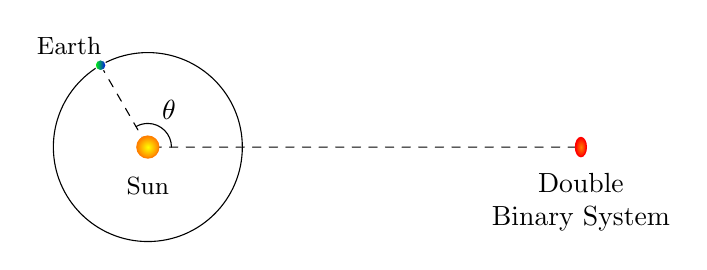
\begin{tikzpicture}[line cap=round, line join=round]
%		%Grid
%		\draw[thin, dotted] (0,0) grid (8,8);
%		\foreach \i in {1,...,8}
%		{
%			\node at (\i,-2ex) {\i};	
%		}
%		\foreach \i in {1,...,8}
%		{
%			\node at (-2ex,\i) {\i};	
%		}
%		\node at (-2ex,-2ex) {0};
		
		%Coordinates
		\coordinate (sun) at (1.5,3);
		\coordinate (earth) at ($(sun)+(120:\radius)$);
		\coordinate (binary system) at (7,3);
		
		%Orbit
		\draw (sun) circle (\radius);
		
		%Lines
		\draw[dashed] (earth) -- (sun) -- (binary system);
		
		%Bodies
		\draw[inner color = yellow, outer color = orange, draw = orange] (sun) circle (4pt);
		\draw[left color = green, right color = blue, draw=white] (earth) circle (2pt);
		\draw[inner color = orange, outer color = red, draw=red, rotate=90] (binary system) ellipse (3.5pt and 2pt);
		
		%Angles
		\pic[draw, "$\theta$", angle eccentricity=1.8, angle radius=0.3cm] {angle = binary system--sun--earth};
		
		%Nodes
		\node[shift={(0,-0.5)}] at (sun) {\small Sun};
		\node[shift={(-0.4,+0.25)}] at (earth) {\small Earth};
		\node[shift={(0,-0.7)}, align=center] at (binary system) {Double\\Binary System};
		
	\end{tikzpicture}
\end{document}
